\documentclass[12pt, oneside]{article} 
\usepackage{amsmath, amsthm, amssymb, calrsfs, wasysym, verbatim, bbm, color, graphics, geometry, multicol}

\usepackage[hidelinks]{hyperref} % Enables hyperlinks without borders
\usepackage{bookmark} % Optional, improves PDF bookmarks
\usepackage{graphicx}
\graphicspath{ {./screenshots/} }

\geometry{tmargin=.75in, bmargin=.75in, lmargin=.75in, rmargin = .75in}  

\newcommand{\ra}{$\rightarrow$ }

\title{COMP 421 - Database Systems\\
        \large Project 2: Creating and Working with Your Database}
\author{Group 99: Luca Mitran, Nicholas Imperioli, Ping-Chieh Tu}
\date{March 10$^{\text{th}}$ 2025}


\begin{document}

\maketitle
\section{Relational Schema}
\begin{tabular}{l@{}l}
    \texttt{Developer(} & \texttt{\underline{did},}\\
                         & \texttt{dname NOT NULL,}\\
                         & \texttt{demail NOT NULL,}\\
                         & \texttt{dphone,}\\
                         & \texttt{PRIMARY KEY (did))}
\end{tabular}

\begin{tabular}{l@{}l}
    \texttt{Publisher(} & \texttt{\underline{pid},}\\
                         & \texttt{pname NOT NULL,}\\
                         & \texttt{pemail NOT NULL,}\\
                         & \texttt{pphone,}\\
                         & \texttt{PRIMARY KEY (pid))}
\end{tabular}

\begin{tabular}{l@{}l}
    \texttt{Game(} & \texttt{\underline{gid},}\\
                    & \texttt{date NOT NULL,}\\
                    & \texttt{rating,}\\
                    & \texttt{price NOT NULL,}\\
                    & \texttt{gname NOT NULL,}\\
                    & \texttt{PRIMARY KEY (gid))}
\end{tabular}

\begin{tabular}{l@{}l}
    \texttt{Category(} & \texttt{\underline{name},}\\
                        & \texttt{PRIMARY KEY (cname))}
\end{tabular}

\begin{tabular}{l@{}l}
    \texttt{Users(} & \texttt{\underline{uid},}\\
                     & \texttt{uemail NOT NULL,}\\
                     & \texttt{password NOT NULL,}\\
                     & \texttt{PRIMARY KEY (uid))}
\end{tabular}

\begin{tabular}{l@{}l}
    \texttt{BillingInfo(} & \texttt{\underline{uid},}\\
                           & \texttt{address,}\\
                           & \texttt{uname NOT NULL,}\\
                           & \texttt{payMethod NOT NULL,}\\
                           & \texttt{PRIMARY KEY (uid),}\\
                           & \texttt{FOREIGN KEY (uid) REFERENCES Users)}
\end{tabular}

\begin{tabular}{l@{}l}
    \texttt{Transactions(} & \texttt{\underline{tid},}\\
                            & \texttt{date NOT NULL,}\\
                            & \texttt{amount NOT NULL,}\\
                            & \texttt{status NOT NULL,}\\
                            & \texttt{uid NOT NULL,}\\
                            & \texttt{PRIMARY KEY (tid),}\\
                            & \texttt{FOREIGN KEY (uid) REFERENCES Users)}
\end{tabular}

\begin{tabular}{l@{}l}
    \texttt{Discount(} & \texttt{\underline{gid}, \underline{startDate},}\\
                        & \texttt{endDate NOT NULL,}\\
                        & \texttt{percentOff NOT NULL,}\\
                        & \texttt{PRIMARY KEY (gid, startDate),}\\
                        & \texttt{FOREIGN KEY (gid) REFERENCES Game)}
\end{tabular}

\begin{tabular}{l@{}l}
    \texttt{MakePublish(} & \texttt{\underline{gid}, did NOT NULL, pid NOT NULL,}\\
                           & \texttt{PRIMARY KEY (gid),}\\
                           & \texttt{FOREIGN KEY (gid) REFERENCES Game,}\\
                           & \texttt{FOREIGN KEY (did) REFERENCES Developer,}\\
                           & \texttt{FOREIGN KEY (pid) REFERENCES Publisher)}
\end{tabular}

\begin{tabular}{l@{}l}
    \texttt{Wish(} & \texttt{\underline{uid}, \underline{gid},}\\
                    & \texttt{PRIMARY KEY (uid, gid),}\\
                    & \texttt{FOREIGN KEY (uid) REFERENCES Users,}\\
                    & \texttt{FOREIGN KEY (gid) REFERENCES Game)}
\end{tabular}

\begin{tabular}{l@{}l}
    \texttt{Own(} & \texttt{\underline{uid}, \underline{gid},}\\
                   & \texttt{PRIMARY KEY (uid, gid),}\\
                   & \texttt{FOREIGN KEY (uid) REFERENCES Users,}\\
                   & \texttt{FOREIGN KEY (gid) REFERENCES Game)}
\end{tabular}

\begin{tabular}{l@{}l}
    \texttt{InCart(} & \texttt{\underline{uid}, \underline{gid},}\\
                      & \texttt{PRIMARY KEY (uid, gid),}\\
                      & \texttt{FOREIGN KEY (uid) REFERENCES Users,}\\
                      & \texttt{FOREIGN KEY (gid) REFERENCES Game)}
\end{tabular}

\begin{tabular}{l@{}l}
    \texttt{Friend(} & \texttt{\underline{uid1}, \underline{uid2},}\\
                      & \texttt{status NOT NULL,}\\
                      & \texttt{PRIMARY KEY (uid1, uid2),}\\
                      & \texttt{FOREIGN KEY (uid1) REFERENCES Users,}\\
                      & \texttt{FOREIGN KEY (uid2) REFERENCES Users)}
\end{tabular}

\begin{tabular}{l@{}l}
    \texttt{BelongsTo(} & \texttt{\underline{gid}, \underline{cname},}\\
                          & \texttt{PRIMARY KEY (gid, cname),}\\
                          & \texttt{FOREIGN KEY (gid) REFERENCES Game,}\\
                          & \texttt{FOREIGN KEY (cname) REFERENCES Category)}
\end{tabular}

\begin{tabular}{l@{}l}
    \texttt{Buy(} & \texttt{\underline{uid}, \underline{gid}, \underline{tid},}\\
                   & \texttt{PRIMARY KEY (uid, gid, tid),}\\
                   & \texttt{FOREIGN KEY (uid) REFERENCES Users,}\\
                   & \texttt{FOREIGN KEY (gid) REFERENCES Game,}\\
                   & \texttt{FOREIGN KEY (tid) REFERENCES Transactions)}
\end{tabular}
\section{Pending Constraints}

\begin{enumerate}
    \item \textbf{Overlapping Discount Dates}: 
    
        For a given game (\texttt{gid}), discount periods (e.g.,\texttt{startDate} and \texttt{endDate}) shouldn't overlap. Since a game cannot have multiple discounts at the same time, application-level logic can be implemented later to enforce this new constraint.
    
    \item \textbf{Transaction Consistency}:
    
         To make sure a user doesn't rebuy a game they own, a transaction (\texttt{tid}) in the \texttt{Buy} table should directly reference a game (\texttt{gid}) that the user (\texttt{uid}) doesn't already own. Using application-level logic to check the \texttt{Own} table before allowing a transaction to be recorded in the \texttt{Buy} table should be implemented. 
        
    \item \textbf{Friend Relationship Ordering/Reflexivity}:
    
        The current constraint \texttt{CHECK (uid1 != uid2)} only prevents a user from friending themselves, it doesn't prevent duplicate entries for example when \texttt{uid1} and \texttt{uid2} are swapped (e.g., \texttt{(1, 2)} and \texttt{(2, 1)}). Implementing application-level logic allows for only one of the 2 orderings to be possible.
    
    \item \textbf{Game Ownership After Purchase}:

        When a user (\texttt{uid}) buys a game (\texttt{gid}), the game should be added to the \texttt{Own} table automatically. Use application-level logic to automatically do this.  
\end{enumerate}

\section{SQL Queries}
\subsection{Query 1}
We would like to know the game name, release date, developer name, publisher name, number of sales as \texttt{sales} of the best selling games based on the number of people that bought them.\\
SQL query: 
\begin{verbatim}
SELECT g.gname AS game_name, 
       g.date AS release_date, 
       d.dname AS developer_name, 
       p.pname AS publisher_name, 
       COUNT(b.uid) AS sales
FROM Buy b
JOIN Game g ON g.gid = b.gid
JOIN Transactions t ON b.tid = t.tid
JOIN MakePublish m ON m.gid = g.gid
JOIN Developer d ON m.did = d.did
JOIN Publisher p ON m.pid = p.pid
WHERE t.status = 'Completed'
GROUP BY b.gid, g.gname, g.date, d.dname, p.pname
HAVING COUNT(b.uid) >= ALL (SELECT COUNT(uid) FROM Buy GROUP BY gid);
\end{verbatim}
\begin{figure}[h]
    \centering
    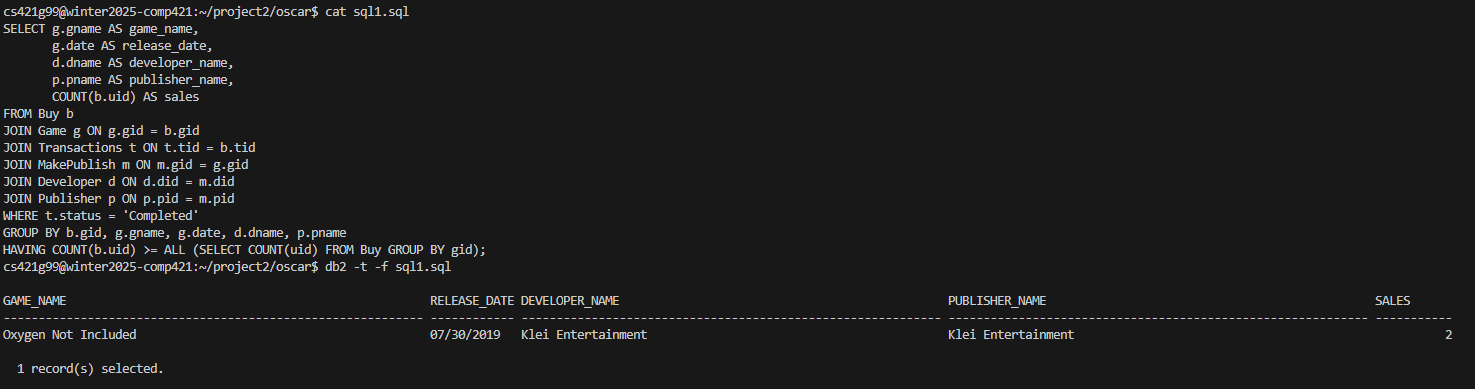
\includegraphics[width=\textwidth]{sql1.png}
\end{figure}
\subsection{Query 2}
We would like to find the best selling game category of each year\\
SQL query:\label{sql:2}
\begin{verbatim}
WITH CategorySales AS (
    SELECT YEAR(t.date) as year, bt.cname, COUNT(b.uid) AS sales
    FROM Buy b
    JOIN Transactions t ON t.tid = b.tid
    JOIN BelongsTo bt ON bt.gid = b.gid
    WHERE status = 'Completed'
    GROUP BY YEAR(t.date), bt.cname
),
Ranks AS (
    SELECT year, cname, sales,
        RANK() OVER(
        PARTITION BY year
        ORDER BY sales DESC
        ) as rank
    FROM CategorySales
)
SELECT year, cname FROM Ranks
WHERE rank = 1;
\end{verbatim}
\begin{figure}[h]
    \centering
    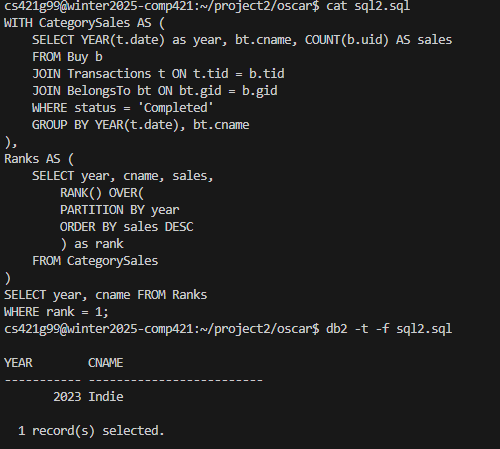
\includegraphics[scale=0.5]{sql2.png}
\end{figure}
\subsection{Query 3}
We each user to receive a list of what their friends last bought game was as a list of game recommendations.\\
SQL query:\label{sql:3}
\begin{verbatim}
WITH FriendWith (user, friend) AS (
    SELECT uid1 AS user, uid2 AS friend
    FROM Friend
    WHERE status = 'Accepted'
    UNION
    SELECT uid2 AS user, uid1 AS friend
    FROM Friend
    WHERE status = 'Accepted'
),
LastBought (user, game_name, rank) AS (
    SELECT b.uid AS user, g.gname AS game_name,
    RANK () OVER (
        PARTITION BY b.uid
        ORDER BY t.date DESC
    ) as rank
    FROM Buy b
    JOIN Game g ON b.gid = g.gid
    JOIN Transactions t ON b.tid = t.tid
    WHERE t.status = 'Completed'
)
SELECT u.uid, COALESCE(lb.game_name, 'None') AS recommandations
FROM Users u
LEFT JOIN FriendWith fw ON u.uid = fw.user
LEFT JOIN LastBought lb ON fw.friend = lb.user AND lb.rank = 1
ORDER BY u.uid;
\end{verbatim}
\begin{figure}[h]
    \centering
    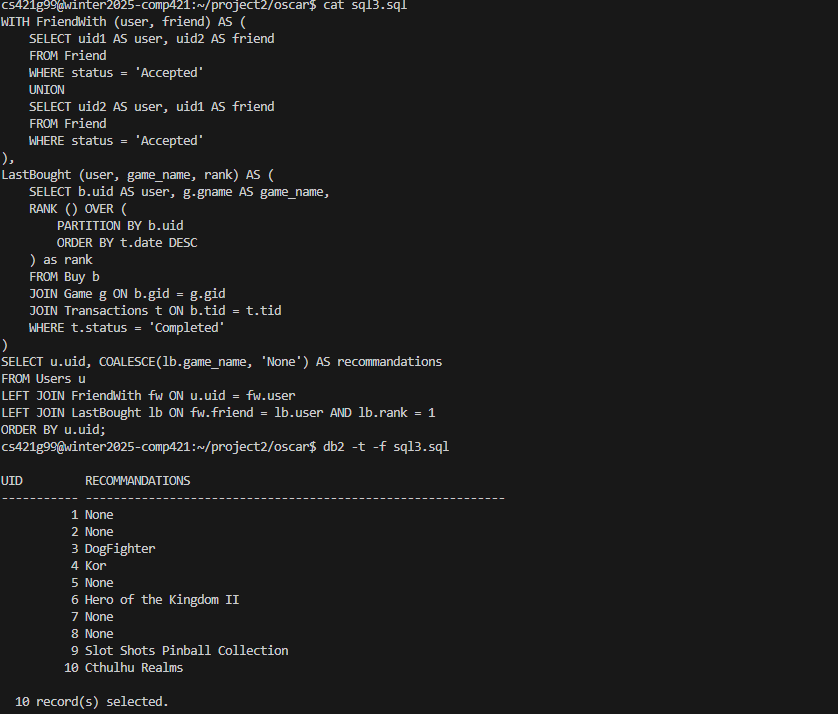
\includegraphics[scale=0.4]{sql3.png}
\end{figure}
\subsection{Query 4}
We would like to give each user a recommended game category based on the games on their wishlist.\\
SQL query:\label{sql:4}
\begin{verbatim}
WITH WishCategory AS (
    SELECT u.uid, bt.cname, COUNT(bt.cname) as count
    FROM Users u
    LEFT JOIN Wish w ON w.uid = u.uid
    JOIN BelongsTo bt ON w.gid = bt.gid
    GROUP BY u.uid, bt.cname
),
Ranks AS (
    SELECT uid, cname, 
    RANK () OVER (
        PARTITION BY uid
        ORDER BY count DESC, cname ASC
    ) as rank
    FROM WishCategory
)
SELECT u.uid, COALESCE(r.cname, 'None') AS recommandations
FROM Users u
LEFT JOIN Ranks r ON u.uid = r.uid AND r.rank = 1
ORDER BY u.uid;
\end{verbatim}
\begin{figure}[h]
    \centering
    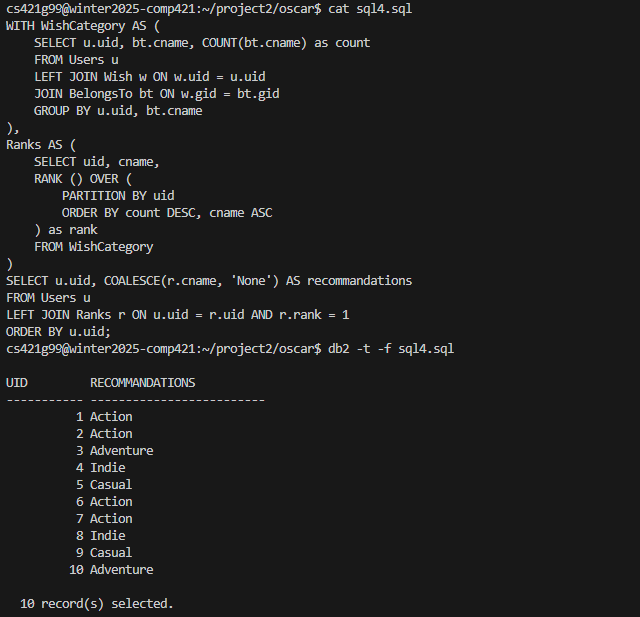
\includegraphics[scale=0.45]{sql4.png}
\end{figure}
\subsection{Query 5}
We would like to give each user a list of games that their friends have on their wishlist\\
SQL query:
\begin{verbatim}
WITH FriendWith (user, friend) AS (
    SELECT uid1 AS user, uid2 AS friend
    FROM Friend
    WHERE status = 'Accepted'
    UNION
    SELECT uid2 AS user, uid1 AS friend
    FROM Friend
    WHERE status = 'Accepted'
)
SELECT fw.user, fw.friend, g.gname AS wish_game
FROM FriendWith fw
JOIN Wish w ON w.uid = fw.friend
JOIN Game g ON w.gid = g.gid
ORDER BY fw.user;
\end{verbatim}
\begin{figure}[h]
    \centering
    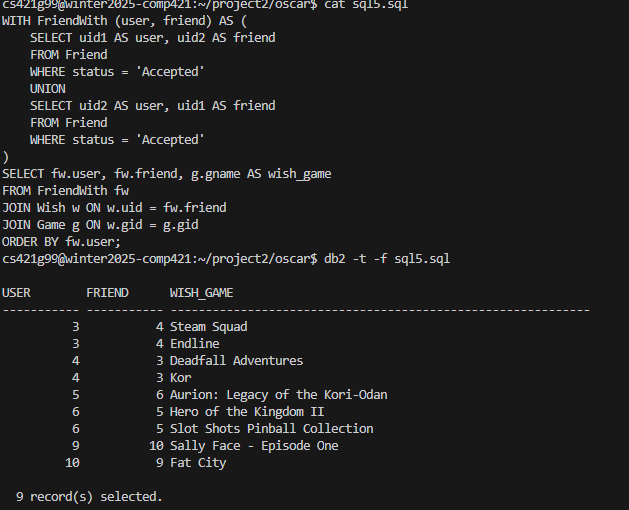
\includegraphics[scale=0.6]{sql5.png}
\end{figure}
\section{SQL Modification}
\subsection{Mod 1}
There is a 40\% discount for 7 days on all games in the Action category that have never had a discount before.\\
SQL query:
\begin{verbatim}
INSERT INTO Discount (gid, startDate, endDate, percentOff)
SELECT b.gid, 
       CURRENT_DATE as startDate,
       CURRENT_DATE + 7 as endDate,
       40 as percentOff
FROM BelongsTo b
WHERE b.cname = 'Action'
AND NOT EXISTS (
    SELECT * FROM Discount d WHERE d.gid = b.gid
);
\end{verbatim}
\begin{figure}[h]
    \centering
    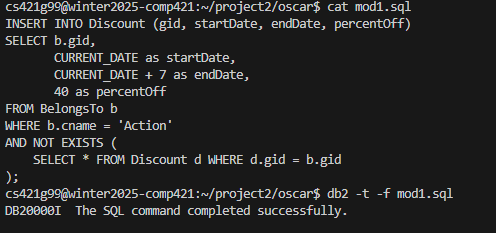
\includegraphics[scale=0.7]{mod1.png}
\end{figure}
\subsection{Mod 2}
The Company Rockstar Games is having a price increase of 10\$ on all of their games.\\
SQL query:
\begin{verbatim}
UPDATE Game g
SET g.price = g.price + 10
WHERE g.gid IN (
    SELECT mp.gid
    FROM MakePublish mp
    JOIN Publisher p ON p.pid = mp.pid
    WHERE p.pname = 'Rockstar Games'
);
\end{verbatim}
\begin{figure}[h]
    \centering
    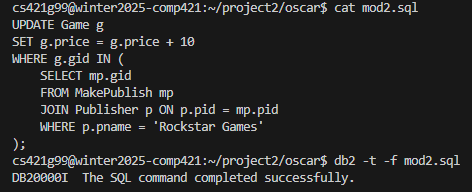
\includegraphics[scale=0.7]{mod2.png}
\end{figure}
\section{Views}
\subsection{View 1}

BasicGameInfo is a simple view that selects budget games from the Game table, specifically those priced under \$20.00. This view provides easy access to affordable games in the marketplace, which is useful for customers looking for budget options. \\

\noindent SQL Query: 
\begin{verbatim}
CREATE VIEW
BasicGameInfo AS
SELECT gid, gname, date, price
FROM Game
WHERE price < 20.00;
\end{verbatim}

% image showing the view creation, query, insert 
\begin{figure}[h]
    \centering
    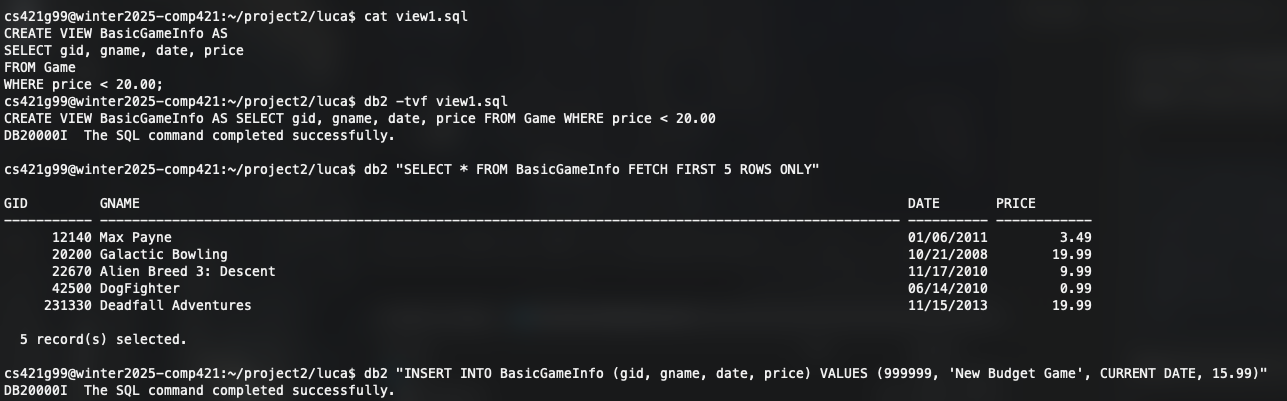
\includegraphics[width=\textwidth]{view1.png}
    \caption{Creation of BasicGameInfo view and results of query and insert}
\end{figure}

The insert operation on this view is successful because BasicGameInfo is a simple view over a single table (Game) with no complex joins or aggregations. The insert operation maps directly to an insert on the underlying Game table, and all necessary columns have valid values.

\subsection{View 2}

GamePurchaseDetails is a complex view that joins multiple tables (Game, Buy, Transactions, and Users) to provide comprehensive information about game purchases. It includes game details, purchase dates, payment amounts, and buyer information for completed transactions. \\

\noindent SQL Query: 

\begin{verbatim}
CREATE VIEW GamePurchaseDetails AS
SELECT
g. gid,
g. gname, g-price,
t.date AS purchase_date,
t. amount AS paid_amount,
u. uid,
u. uemail AS buyer_email
FROM
Game g
JOIN
Buy b ON g-gid = b.gid
JOIN
Transactions t ON b.tid = t.tid
JOIN
Users u ON b.uid = u.uid
WHERE
t. status = 'Completed';
\end{verbatim}

\begin{figure}[h]
    \centering
    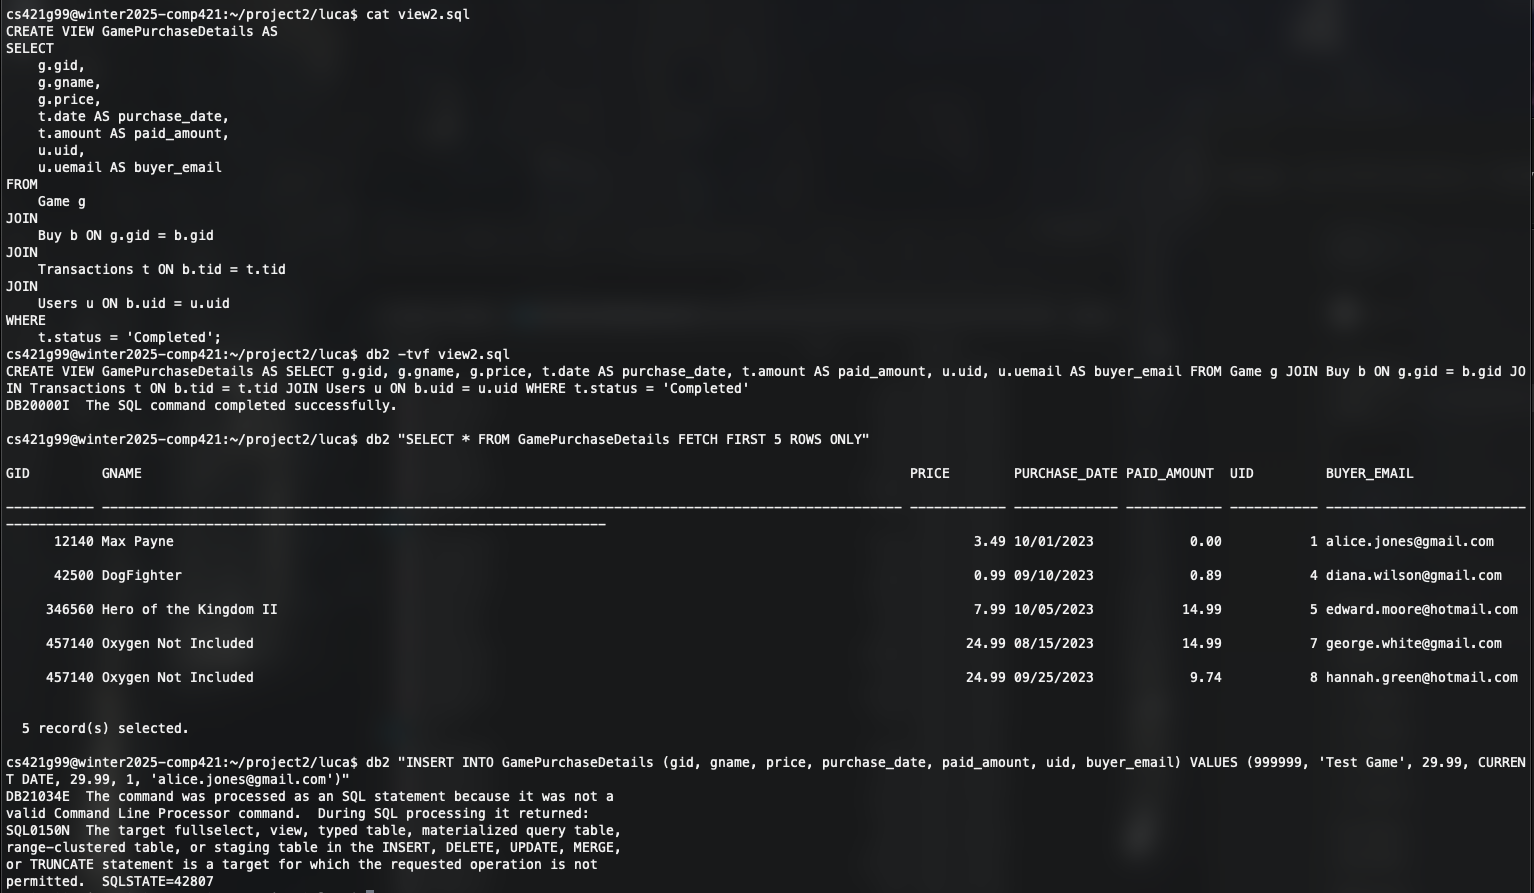
\includegraphics[width=\textwidth]{view2.png}
    \caption{Creation of GamePurchaseDetails view and results of query and insert}
\end{figure}

The insert operation on this view fails with an SQL0150N error because GamePurchaseDetails is a complex view that joins multiple tables. According to DB2's rules for view insertability, inserts are not permitted on views that include joins, as the database cannot automatically determine how to distribute the inserted data across the underlying tables.

\section{Check Constraints}

\subsection{Check 1}

This constraint ensures that discount percentages in the Discount table are always greater than 0 and less than or equal to 100\%. This is a critical business rule for the video game marketplace as it prevents invalid discount values that could cause pricing errors. \\

\noindent SQL Query: 

% image showing the constraint statement, execution, violation test
\begin{verbatim}
ALTER TABLE Discount
ADD CONSTRAINT check_discount_range
CHECK (percentoff > 0 AND percentoff <= 100);
\end{verbatim}

When a user attempts to insert a discount percentage that exceeds 100\%, the database rejects the operation and returns an SQL0545N error indicating that the row does not satisfy the check constraint.

\subsection{Check 2}

This constraint restricts the status field in the Friend table to only contain one of the predefined values: Pending, Accepted, Blocked, or Rejected. This maintains data consistency in the friend relationship system and prevents invalid status values. \\

\noindent SQL Query: 

\begin{verbatim}
ALTER TABLE Friend
ADD CONSTRAINT check_friend_status
CHECK (status IN ('Pending',
'Accepted', 'Blocked',
'Rejected'));
\end{verbatim}

\begin{figure}[h]
    \centering
    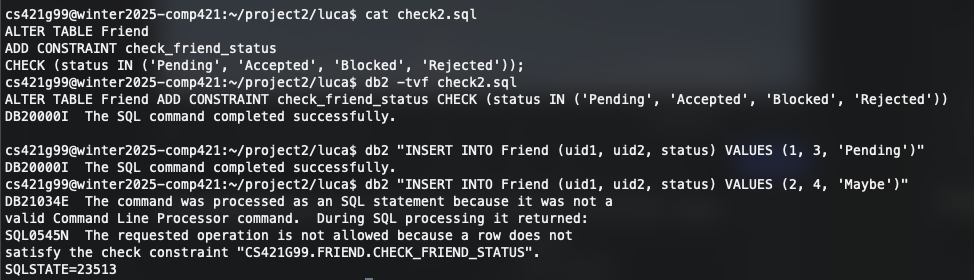
\includegraphics[width=\textwidth]{check2.png}
    \caption{Implementation of the friend status constraint, results of inserting record which violates the constraint}
\end{figure}

The constraint successfully prevents users from entering undefined status values in the Friend table, returning an SQL0545N error when attempting to use 'Maybe' as a status, which is not in the allowed list.

\section{Creativity}
\subsection{Real data sets}
We used the dataset found on Kaggle\footnote{\href{https://www.kaggle.com/datasets/fronkongames/steam-games-dataset}{https://www.kaggle.com/datasets/fronkongames/steam-games-dataset}} to generate the data for 100 games. \texttt{loaddata.py} shows how the data was scraped from the database and the outputs are also provided in the folder \textbf{Scraped Data}. The size of the raw data file is too large to to include in the submission as it contains 1000s of games; Using the link in the footnote will allow you to access the data.

\subsection{Advanced SQL Features}
In \hyperref[sql:2]{SQL 2}, \hyperref[sql:3]{SQL 3} and \hyperref[sql:4]{SQL 4}, we used \texttt{RANK() OVER ([partition] ORDER BY order) AS rank}. This will rank the tables by order (from 1 to n), the partition is like \texttt{GROUP BY}. In \hyperref[sql:2]{SQL 2}, it groups the sales by year and rank in each year. In \hyperref[sql:3]{SQL 3}, it groups the games bought and rank for each user by the time they bought it. In \hyperref[sql:4]{SQL 4}, it groups the games category and rank for each user by the count of the category in their wishlist. The function \texttt{COALESCE(...)} will return the first non-null element in the list.For example in \hyperref[sql:3]{SQL 3}, \texttt{COALESCE(lb.game\_name, 'None')} returns \texttt{lb.game\_name} and if it is not NULL, and will return \texttt{`None'} if \texttt{lb.game\_name} is NULL.

\section{Teamwork}

We communicated regularly during the project's availability with meetings at least once a week. The work was divided evenly among us where one person worked on parts 3 and 4, one worked on parts 5 and 6, and the last person worked on parts 7 and 8. Part 2 was a copy paste of the relational schema from deliverable 1 as nothing changed there and the creativity section was a joint effort between all members. After a section was completed, we would join a meeting and discuss any changes/challenges that were present and looked towards solving them. Once every section was complete we had a final meeting verifying that all requirements were met and that the work was to an acceptable standard.
\end{document}
